\documentclass[12pt,usletter,english]{article}
\usepackage[utf8]{inputenc}
\usepackage{graphicx}
\usepackage{amsmath}
\usepackage{amssymb}
\usepackage{subcaption}
\usepackage[font={small}]{caption}
\usepackage{fancyhdr}
\usepackage{float}
\usepackage{listings}

\pagestyle{fancy}
\lhead{Problem Set 1} \rhead{Deepthi Gorthi}

\begin{document}
\title{PS1: Introduction to Probablity and Statistics} \author{Deepthi Gorthi\\ AY250: Stellar Populations} \maketitle

\noindent \textbf{Problem 1.} \\ 

(a) In 1995, they introduced blue M\&M's.  Before then, the color mix
in a bag of plain M\&M's was 30\% brown, 20\% yellow, 20\% red, 10\%
green, 10\% orange, and 10\% tan.  Afterward, it was 24\% blue, 20\%
green, 16\% orange, 14\% yellow, 13\% red, 13\% brown.

Suppose there are two bags of M\&M's, one from 1994 and one from 1996
and you are randomly given one M\&M from each bag.  One is yellow, one
is green.  Using Bayes's theorem and a probability table to determine
the \underline{relative} probability that the yellow M\&M came from
the 1994 bag. \\

(b) Evaluate the ``Evidence'' and determine the \underline{normalized}
probability that the yellow M\&M came from the 1994 bag. \\

\noindent \textbf{Solution:} \\

(a) The given distribution of M\&M's can be summarized as follows:
%% +------+-----+-----+
%% |Colour|1994 |1996 |
%% +------+-----+-----+
%% |Brown |0.3  |0.13 |
%% +------+-----+-----+
%% |Yellow|0.2  |0.14 |
%% +------+-----+-----+
%% |Red   |0.2  |0.13 |
%% +------+-----+-----+
%% |Green |0.1  |0.2  |
%% +------+-----+-----+
%% |Orange|0.1  |0.16 |
%% +------+-----+-----+
%% |      |0.1  |0.24 |
%% +------+-----+-----+

\begin{center}
\label{tab:mm}
\begin{tabular}{|l|l|l|}
\hline
Colour & 1994 & 1996 \\
\hline
Brown & 0.3 & 0.13 \\
\hline
Yellow & 0.2 & 0.14 \\
\hline
Red & 0.2 & 0.13 \\
\hline
Green & 0.1 & 0.2 \\
\hline
Orange & 0.1 & 0.16 \\
\hline
Other & 0.1 & 0.24 \\
\hline
\end{tabular}
\end{center}

Given data: One M\&M was drawn from each sample and one of them is
yellow and another green. To evaluate the relative probablity that the
yellow M\&M was drawn from the 1994 bag (and hence the green from the
1996 bag), define the two hypothesis as:\\

\noindent$H_1$: Yellow M\&M- 1994 bag, Green M\&M- 1996 bag.\\

\noindent$H_2$: Yellow M\&M- 1996 bag, Green M\&M- 1994 bag.\\

Since we have no prior knowledge about either hypothesis, we should
begin with flat priors- either hypothesis is equally likely. For
probability of the data given the hypothesis we can multiply the
probabilities of drawing the green and yellow M\&Ms from the
respective bag, since they are independent events.
%% +----------+-------+------------+-----------+
%% |Hypothesis|P(H)   |P(D|H)      |P(D|H)*P(H)|
%% |          |       |            |           |
%% +----------+-------+------------+-----------+
%% |$H_1$     |1/2    |(0.2)*(0.2) |0.02       |
%% |          |       |            |           |
%% +----------+-------+------------+-----------+
%% |$H_2$     |1/2    |(0.14)*(0.1)|0.007      |
%% |          |       |            |           |
%% +----------+-------+------------+-----------+

\begin{center}
\begin{tabular}{|l|l|l|l|}
\hline
Hypothesis & P(H) & P(D$|$H) & P(D$|$H)*P(H) \\
 & & & \\
\hline
$H_1$ & 1/2 & (0.2)*(0.2) & 0.02 \\
 & & & \\
\hline
$H_2$ & 1/2 & (0.14)*(0.1) & 0.007 \\
 & & & \\
\hline
\end{tabular}
\end{center}

The relative probability that the yellow M\&M was drawn from the 1994
bag is \fbox{0.02}.\\

\noindent(b) The `evidence' is also the probability of the data given
all the possible hypotheses. This can be obtained by summing over the
likelihoods of all the hypotheses.
\begin{equation}
  P(D) = 0.02+0.007 = 0.027
\end{equation}

\noindent Hence the normalized probability that the yellow M\&M came
from the 1994 bag is:

\begin{equation}
  P(H_1|D) = \frac{P(D|H_1)*P(H_1)}{P(D)} = \frac{0.02}{0.027} \sim
  74\%
\end{equation}

The normalized probability of our hypothesis that the yellow M\&M was
drawn from the 1994 bag is \fbox{74\%}.

\newpage

\noindent \textbf{Problem 2.} \\ 

Using notes from class, code up your own Metropolis-Hastings (M-H)
MCMC sampler.  Although it is technically impossible to prove that an
MCMC sampler definitively converges (this would require infinite
runtime), a simple sanity test it is to sample from a one dimensional
Gaussian distribution:
\begin{equation}
P(x)= \frac{1}{\sqrt{2\pi\sigma^2}} e^\frac{-(\mu-x)^2}{2\sigma^2}
\end{equation}

\noindent where $\mu$ and $\sigma$ are values you choose, and $x$
values are generated by your M-H sampler.  The density of samples
should trace the input distribution.  For example, if you select
$\mu=5$ and $\sigma=1$, the density of samples for $x$ should be a 1d
Gaussian with these values (perhaps modulo a normalization
constant). Make plots that qualitatively demonstrate convergence of
your sampler to a steady state (e.g., lnP vs. $x$, lnP vs. step
number) and a plot that shows your samples relative to the true
distribution. Your choice in step size should yield an acceptance
fraction between $\sim$0.25 and 0.5. \\

\noindent \textbf{Solution}\\

The Metropolis-Hastings Algorithm that I wrote up to sample the given
gaussian function is included in this repository as
\fbox{\texttt{mcmc\_sampler.py}}

The proposal density was chosen to be a Gaussian function centered
around the current point. The width of the gaussian was found to
affect the step size and hence the acceptance rate of the sampler. It
was fixed by hit and trial till an acceptance rate $\sim 0.32$ was
obtained.

\begin{figure}[!h]
  \centering 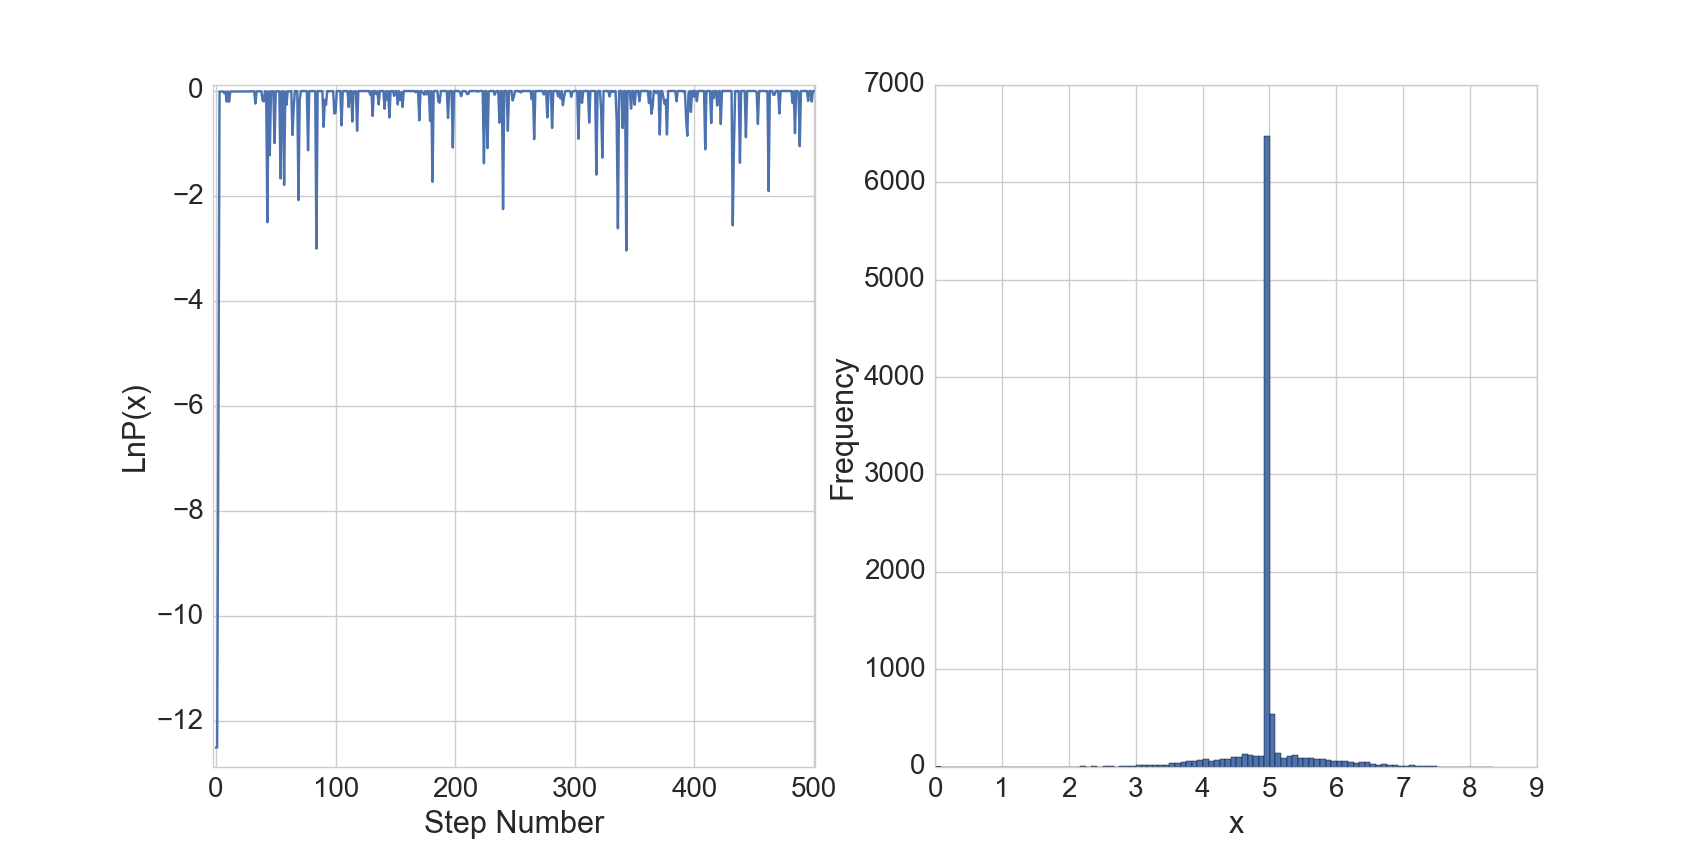
\includegraphics[width=15cm]{diagnostics.png}
  \caption{Diagnostic plots of the MCMC sampler to demostrate
    convergence of the Markov chain. The log likelihood probability
    distribution is sampled both at high and low probability areas, as
    shown in panel(1). Only the first 500 samples are shown for
    illustration. Panel(2) shows that the sampler is predominantly in
    the high probability region around the peak of the gaussian as
    compared to the wings.
    \label{fig:diagnostics}}
\end{figure}

\begin{figure}[!h]
  \centering 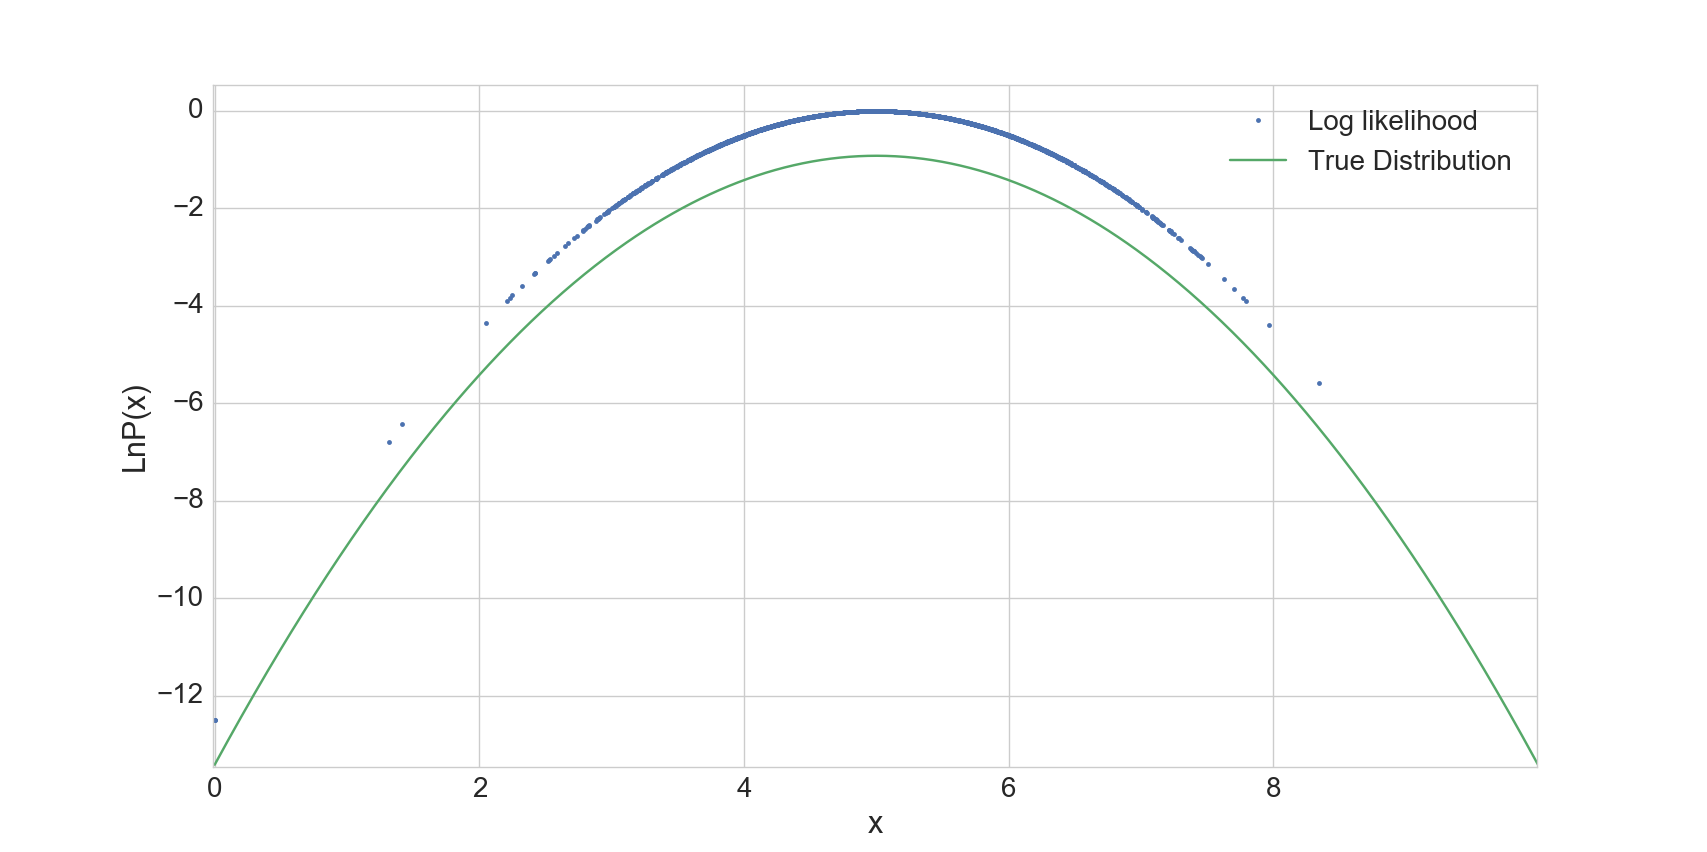
\includegraphics[width=15cm]{dist_mcmc.png}
  \caption{The figure shows the PDF reconstructed from the Markov
    chain against the actual log probability distribution of the given
    Gaussian. The sampler suceeds in reconstructing the PDF modulo a
    normalization constant.
    \label{fig:hist}}
\end{figure}

The Markov chain's convergence can be see from the plot of
figure~\ref{fig:diagnostics}. The left panel shows that the walker is
moving between high and low probability regions randomly, and the
right panel shows that over the simulation time the walker spends more
time in the high probability area around the peak of the gaussian as
compared to the wings.

Finally, figure~\ref{fig:hist} shows that the PDF can be reconstructed
very accurately, modulo a normalization factor, using the MCMC
sampler.

\newpage

\noindent \textbf{Problem 3.} \\ 

\noindent Using a probabilistic framework, write code that fits a
straight line (i.e., $y=mx+b$) to fake data (i.e., data points and
error bars).  You will need to write a function that simulates fake
data that includes Gaussian noise and an arbitrary number of
points. \\

(a) Assume true values of $m=5$, $b=-2$. Use the M-H MCMC sampler you
wrote in problem 2 to infer the true values of $m$ and $b$ for 10,
100, and 1000 data points.  Choose a modest amplitude for your
uncertainties and clearly indicate your choice. For simplicity, you
may assume top hat (`flat') priors for $m$ and $b$. Make relevant
diagnostic plots to indicate convergence, and plot your final results
using \texttt{corner.py}. \\

(b) Repeat part (a), but replace your M-H sampler with
\texttt{emcee}. \\

\noindent \textbf{Solution}\\

A program to simulate fake data with $m=5$, $b=-2$ and gaussian
uncertainities, and then to fit this straight line using the MCMC
sampler from the previous problem is included in this repository under
\fbox{\texttt{fit_line.py}}

The simulated fake data is shown in figure~\ref{fig:fakedata}. The
Gaussian uncertainities were drawn from a normal distribution centered
around zero and of width 10. 

\begin{figure}[!h]
  \centering 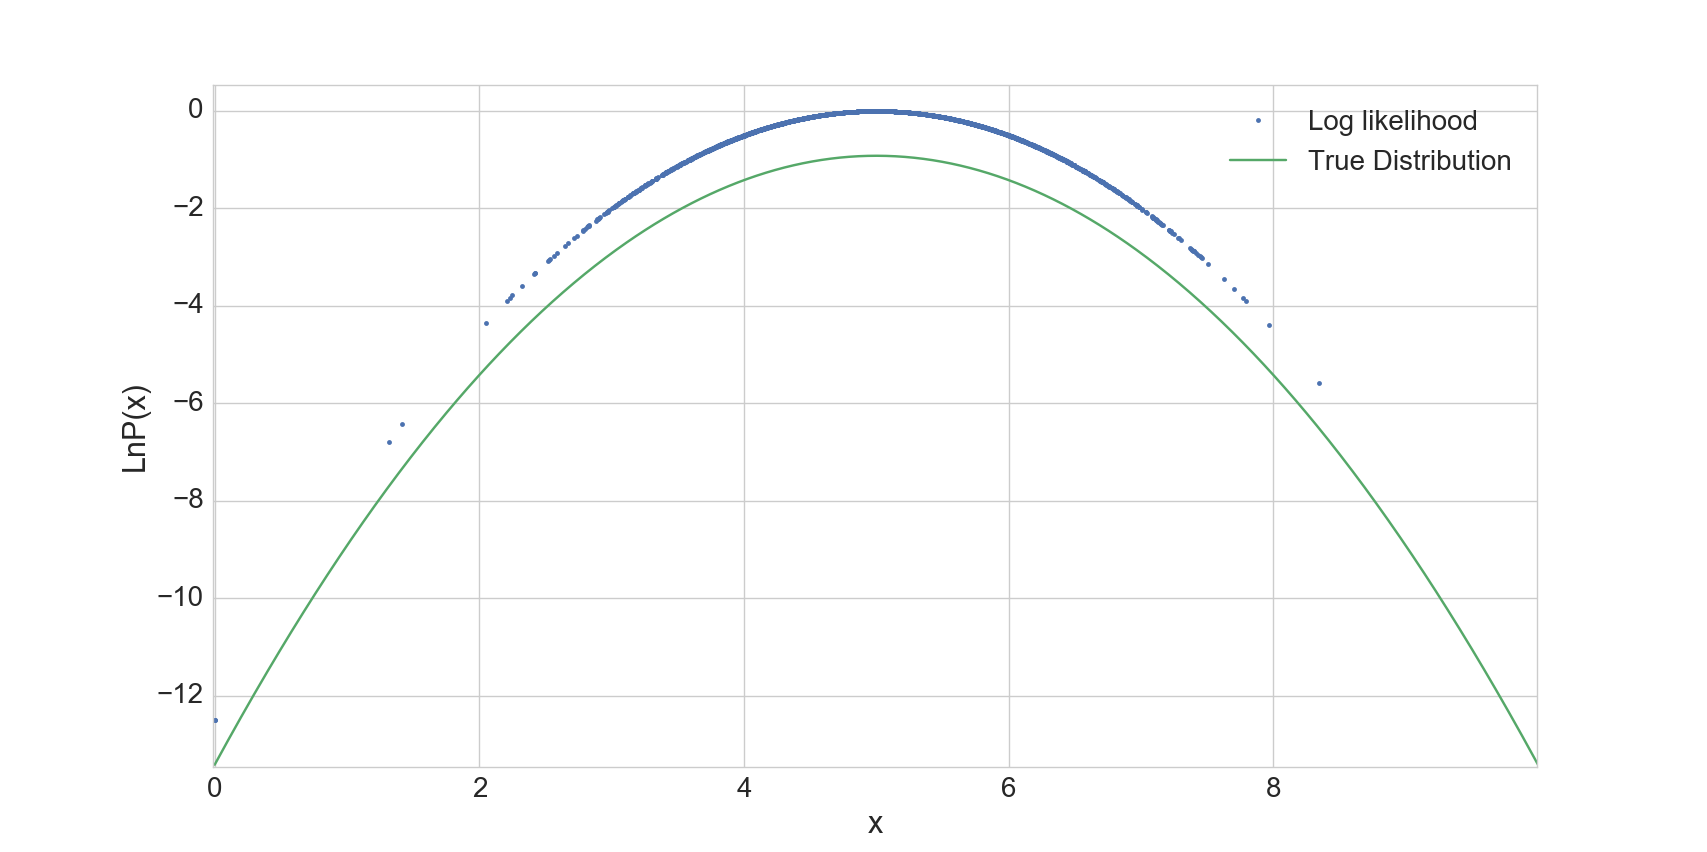
\includegraphics[width=15cm]{dist_mcmc.png}
  \caption{The figure shows the PDF reconstructed from the Markov
    chain against the actual log probability distribution of the given
    Gaussian. The sampler suceeds in reconstructing the PDF modulo a
    normalization constant.
    \label{fig:hist}}
\end{figure}

\end{document}
